\documentclass[../Supercritical_fluid_extraction_of_essential_oil_from_chamomile.tex]{subfiles}
\graphicspath{{\subfix{../Figures/}}}
\begin{document}
	
	\label{CH: Results}
		
	To solve the parameter estimation problem, the single shooting method was used to transform the boundary-value problem into the initial value problem and to formulate the non-linear programming problem. This non-linear optimisation task was tackled using the CasADi framework (\citet{Andersson2018}). Each time series was fitted separately to the model with the linear extraction kinetics (Equation \ref{Model_kinetic_no_sat}). The parameter estimation problem was solved multiple times with varying parameter initial values to identify the global minimum. In the case of linear, two parameters remain to be determined: the partition coefficient $k_m$ and the internal diffusion coefficient $D_i$. \citet{Rahimi2011} analysed the same dataset and reported Peclet numbers between 290 and 400. Large Peclet number suggests that the advection term dominates the mass transfer, and the axial diffusion is negligible, which is one of the modelling assumptions.
		
	\begin{figure}[!h]
		\centering
		\begin{subfigure}{0.9\columnwidth}
			\centering
			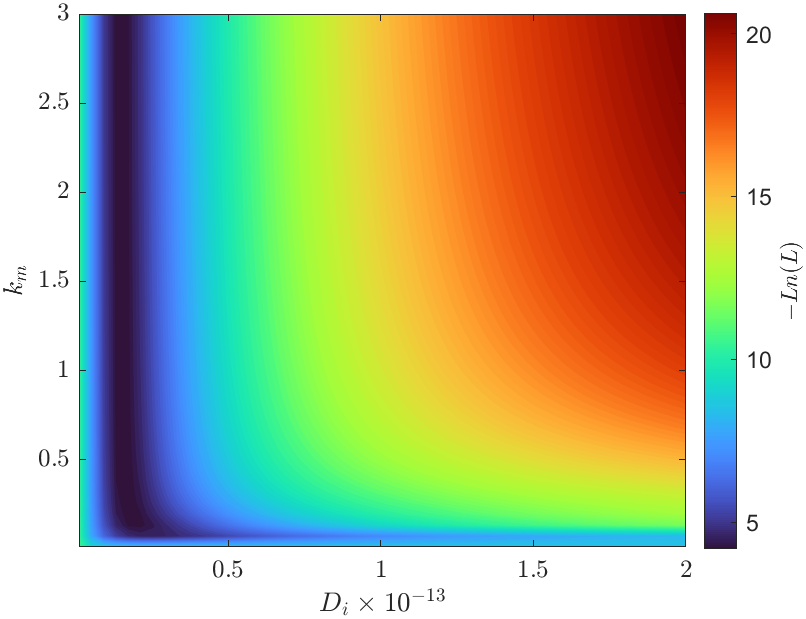
\includegraphics[trim = 0.0cm 0.0cm 0.0cm 0.0cm,clip, width=\columnwidth]{/Results_estimation/Parameter_Space_Linear_Dataset_1.png}
			\caption{The linear kinetic model \\ ~}
			\label{fig: Fit_1_linear}
		\end{subfigure}
		\hfill
		\begin{subfigure}{0.9\columnwidth}
			\centering
			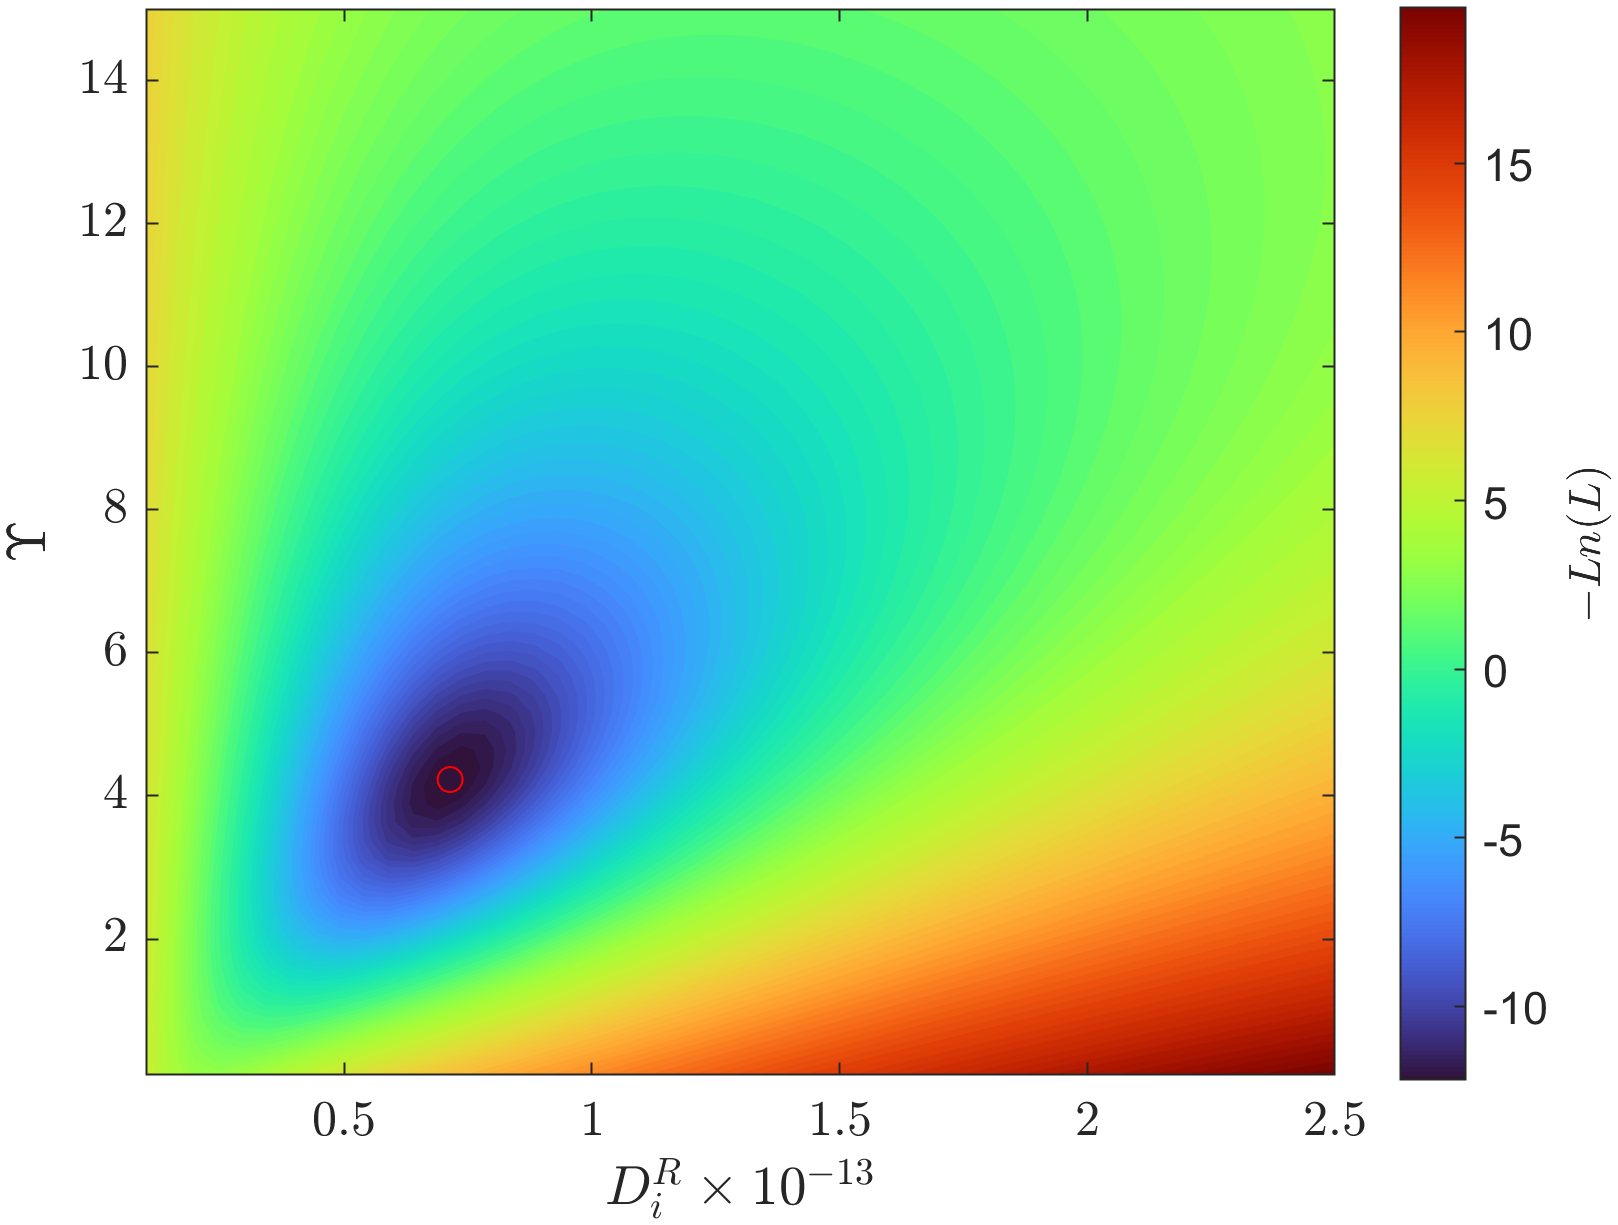
\includegraphics[trim = 0.0cm 0.0cm 0.0cm 0.0cm,clip, width=\columnwidth]{/Results_estimation/Parameter_space_Di_Gamma_dataset_1_org.png}
			\caption{The modified model}
			\label{fig: Fit_1_Di_Gamma}
		\end{subfigure}
		\caption{Parameter space for experiment 1}
		%\label{fig: Fit_Di_Gamma}
	\end{figure}
	
	Figure \ref{fig: Fit_1_linear} shows the parameter space and corresponding values of the cost function for experiment 1 ($40^\circ C$, 100 bar and 6.67$\cdot 10^{-5}$ kg/s). A black-coloured section, in the shape of a vertical stripe at $D_i \approx 0.2$, indicates the minimum values of the cost function $-\ln(L)$. In the direction of $k_m$, the cost function is almost flat, which suggests that any value of $k_m$ above 0.1 fits the data equally well. If $k_m$ can be an arbitrary point, then it can grow to infinity, which suggests that the solvent is far from the saturation, and the model can be simplified. The model reduction can be introduced by considering the limit of $k_m$:
		
	{\footnotesize
		\begin{equation*}
			\begin{split}
				&\lim_{k_m \rightarrow \infty} \left({\color{black}{\color{black} c_s} }(t,z)  - \cfrac{{\color{black}\rho_s}}{{\color{black}k_m}(T(t,z)){\color{black}\rho}(T(t,z),{\color{black}P}(t))}  c_f \right)  = \\
				&= \left({\color{black}{\color{black} c_s} }(t,z)  - \cfrac{\rho_s}{\infty \cdot \rho(T(t,z),P(t))}  {c_f}(t,z) \right) = \left(c_s(t,z) - 0 \right)
			\end{split}
	\end{equation*} }
	
	In the scenario previously discussed, the fitting outcomes were not deemed satisfactory. Building upon the concepts underlying the Broken-and-Intact and Shrinking Core models (detailed in Chapter \ref{CH: Gamma_Function}), the $\gamma$-function is introduced to capture the decreasing extraction kinetics. The correction factor is combined with the simplified linear model, resulting in a two-parameter model ($D_i^R$ and $\Upsilon$) as given by Equation \ref{Model_kinetic}. Figure \ref{fig: Fit_1_Di_Gamma} shows the parameter space and the corresponding cost function values.
		
	\begin{figure}[!h]
		\centering
		\begin{subfigure}{0.9\columnwidth}
			\centering
			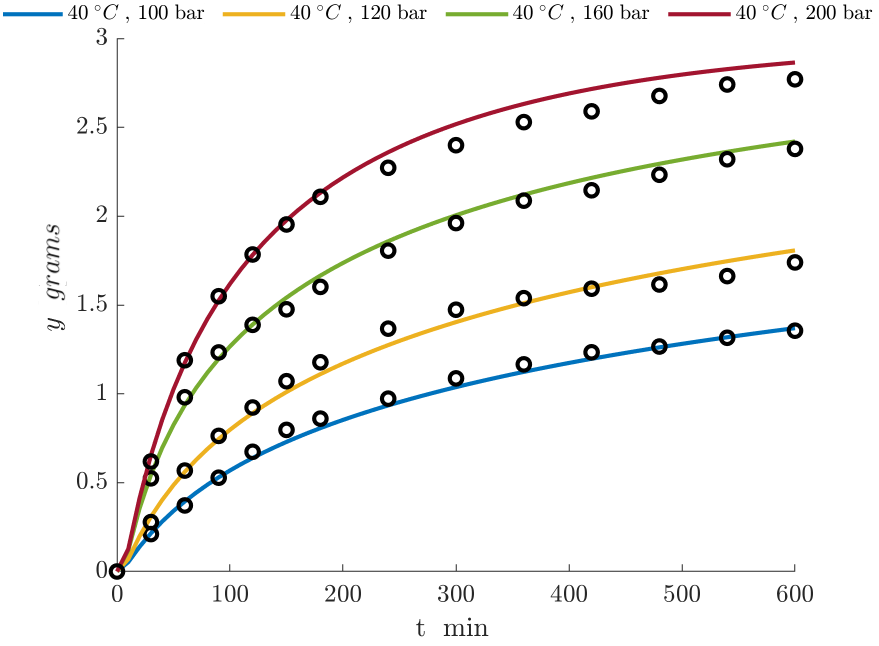
\includegraphics[trim = 0.0cm 0.0cm 0.0cm 0.0cm,clip, width=\columnwidth]{/Results_estimation/Fit_Di_Gamma_1_4_1.png}
			\caption{Parameter estimation results at $6.67\cdot 10^{-5}$ kg/s and temperature of 40 $^\circ C$}
			\label{fig: Fit_1_4_Di_Gamma}
		\end{subfigure}
		\hfill
		\begin{subfigure}{0.9\columnwidth}
			\centering
			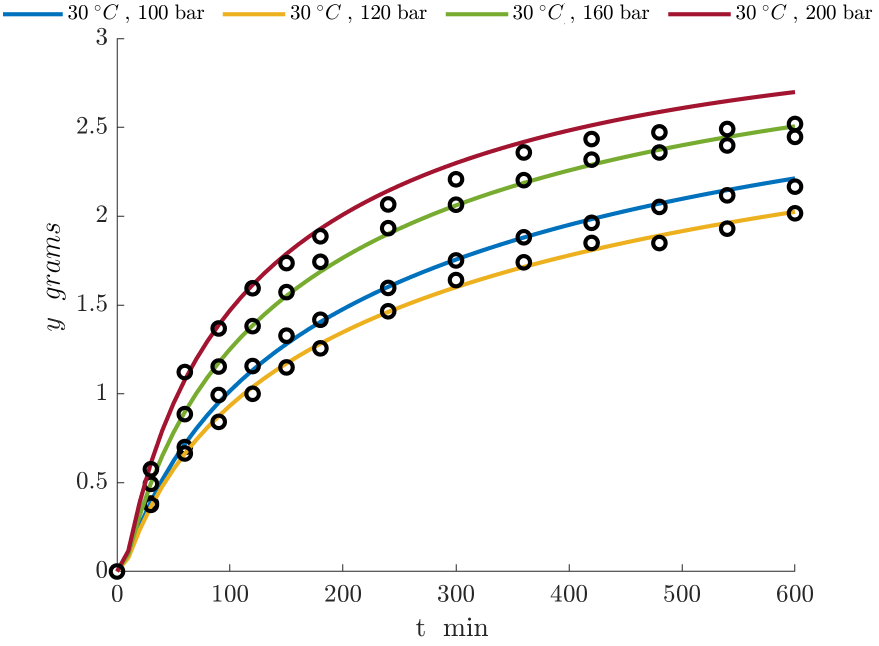
\includegraphics[trim = 0.0cm 0.0cm 0.0cm 0.0cm,clip, width=\columnwidth]{/Results_estimation/Fit_Di_Gamma_5_8_1.png}
			\caption{Parameter estimation results at $6.67\cdot 10^{-5}$ kg/s and temperature of 30 $^\circ C$}
			\label{fig: Fit_5_8_Di_Gamma}
		\end{subfigure}
		\hfill
		\begin{subfigure}{0.9\columnwidth}
			\centering
			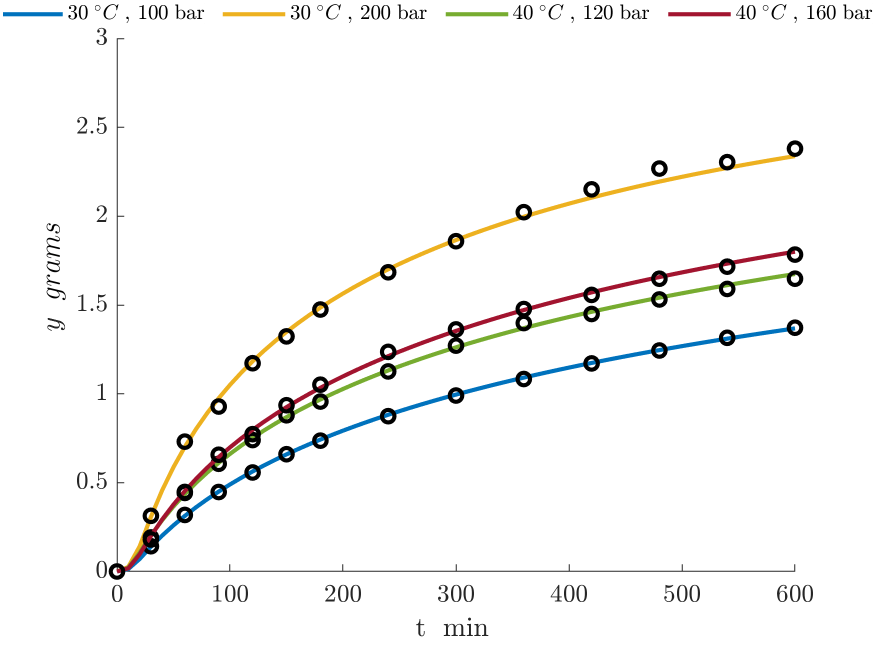
\includegraphics[trim = 0.0cm 0.0cm 0.0cm 0.0cm,clip, width=\columnwidth]{/Results_estimation/Fit_Di_Gamma_9_12_1.png}
			\caption{Results of parameter estimation for experiments at $3.33\cdot 10^{-5}$ kg/s}
			\label{fig: Fit_9_12_Di_Gamma}
		\end{subfigure}
		\caption{Parameter estimation results obtained from the modified model}
		\label{fig: Fit_Di_Gamma}
	\end{figure}
	
	The parameter space for the modified model exhibits a distinct minimum value corresponding to the solution of the parameter estimation problem for experiment 1. The red circle highlights the minimum value of the cost function found by the optimizer. The remaining experiments are fitted to the modified extraction model, and results, presented in Figure \ref{fig: Fit_Di_Gamma}, show good agreement with experimental data. 
		
	The parameter estimation results are combined to analyse the relationship between the obtained parameters and the operating conditions. Unlike traditional methods that employ a combination of Reynolds, Schmidt, and Sherwood numbers to find correlation, the approach in this study leverages the fixed-bed Reynolds number $\left(Re = \frac{2r \cdot \rho_f \cdot u}{\mu}\right)$ as the sole independent variable. Using the Reynolds number has the advantage of considering the influence of all the control variables (temperature, pressure and flow rate), which means it can be uniquely defined by selecting operating conditions.	
	
	\begin{figure}[!h]
		\centering
		\begin{subfigure}{0.9\columnwidth}
			\centering
			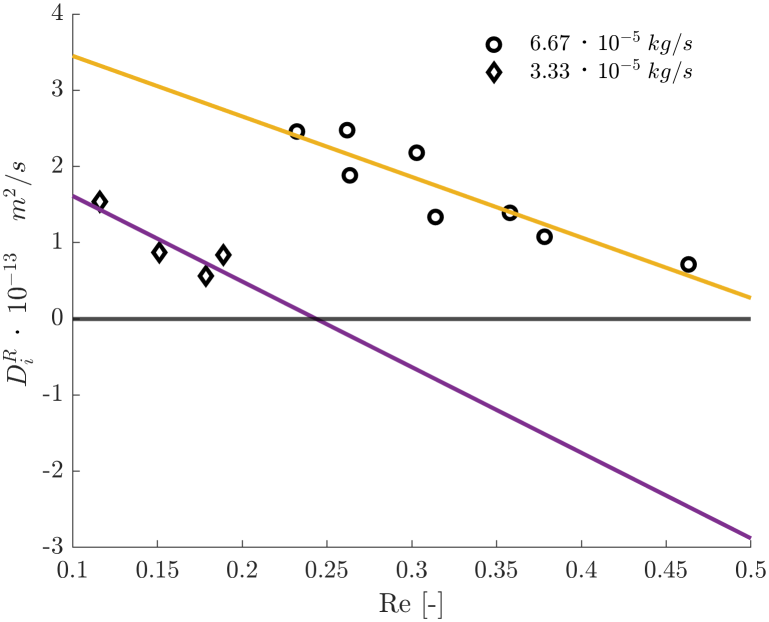
\includegraphics[trim = 0.0cm 0.0cm 0.0cm 0.0cm,clip, width=\columnwidth]{/Results_estimation/Correlation_Di_Re_1.png}
			\caption{Linear regression $D_i^R = f(Re)$}
			\label{fig: Correlations_Di_Re}
		\end{subfigure}
		\hfill
		\begin{subfigure}{0.9\columnwidth}
			\centering
			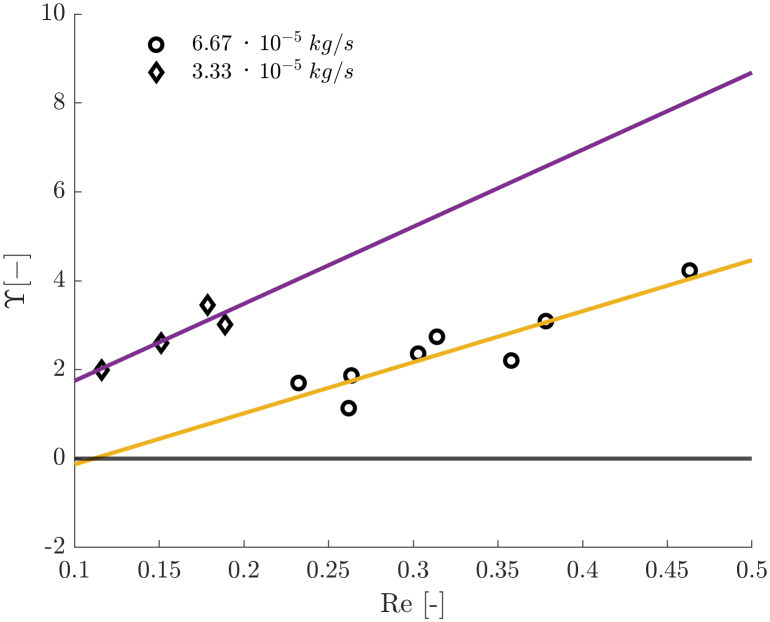
\includegraphics[trim = 0.0cm 0.0cm 0.0cm 0.0cm,clip, width=\columnwidth]{/Results_estimation/Correlation_Gamma_Re_1.png}
			\caption{Linear regression $\Upsilon = f(Re)$}
			\label{fig: Correlations_Gamma_Re}
		\end{subfigure}
		\caption{Linear correlations between parameters}
		%\label{fig: Correlations_surface}
	\end{figure}
	
	In Figures \ref{fig: Correlations_Di_Re} and \ref{fig: Correlations_Gamma_Re}, two distinct data clusters emerge, each corresponding to a different mass flow rate. Despite the linear trends observed in both sets of correlations, the correlations for $D_i^R$ exhibit a decline with increasing $Re$, whereas those for $\Upsilon$ show an upward trend with $Re$. The decrease in $D_i^R$ across each data line can be attributed to higher fluid density and increased mass transfer resistance.
	
	\begin{figure}[!h]
		\centering
		\begin{subfigure}{0.9\columnwidth}
			\centering
			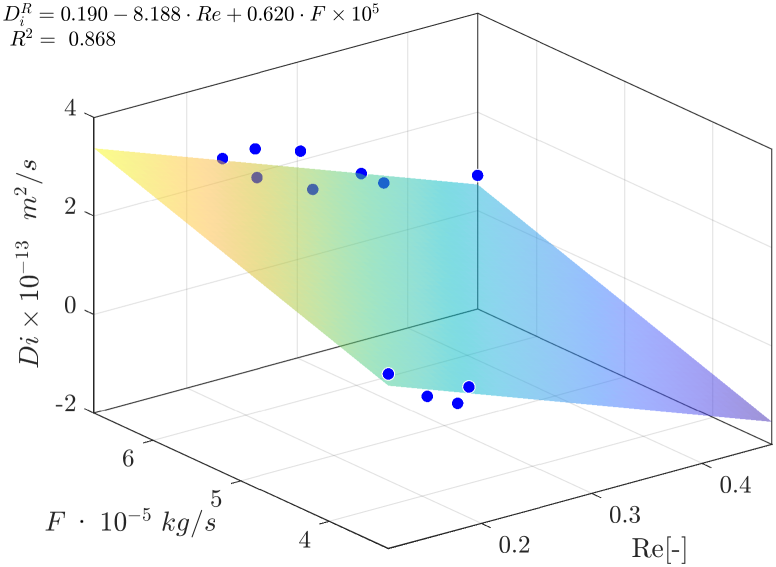
\includegraphics[trim = 0.0cm 0.0cm 0.0cm 0.0cm,clip, width=\columnwidth]{/Results_estimation/Di_Re_F_1.png}
			\caption{Multiple linear regression $D_i^R = f(Re, F)$}
			\label{fig: Correlations_Di_Re_F}
		\end{subfigure}
		\hfill
		\begin{subfigure}{0.9\columnwidth}
			\centering
			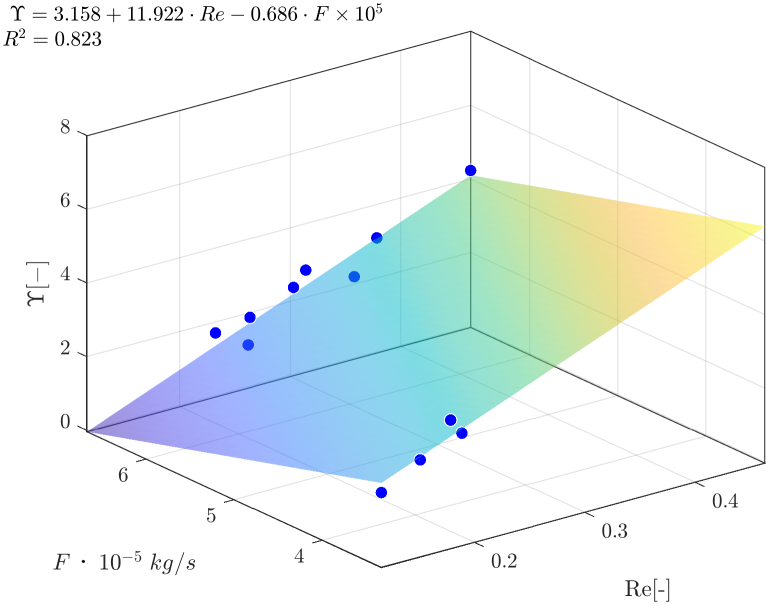
\includegraphics[trim = 0.0cm 0.0cm 0.0cm 0.0cm,clip, width=\columnwidth]{/Results_estimation/Gamma_Re_F_1.png}
			\caption{Multiple linear regression $\Upsilon = f(Re, F)$}
			\label{fig: Correlations_Gamma_Re_F}
		\end{subfigure}
		\caption{Empirical correlations between parameters}
		%\label{fig: Correlations_surface}
	\end{figure}
	
	A more general relationship can be obtained by applying multiple linear regression instead of linear regression. The data clusters in Figure \ref{fig: Correlations_Di_Re} and \ref{fig: Correlations_Gamma_Re} are close to parallel, suggesting that a plane would combine all the data points. The Reynolds number and mass flow rate act as independent variables for $D_i^R$ and $\Upsilon$ as presented in Figures \ref{fig: Correlations_Di_Re_F} and \ref{fig: Correlations_Gamma_Re_F}. The presented correlations are valid in the whole range of investigated operating conditions. The correlations are later tested against the original dataset to show that the correlations can reproduce the results with satisfactory accuracy. Figure \ref{fig: Fit_Di_Gamma_correlation} shows the results of the simulations with incorporated correlations. A good agreement between simulation results and the dataset can be observed. If Figures \ref{fig: Fit_Di_Gamma} and \ref{fig: Fit_Di_Gamma_correlation} are compared, a decrease in the accuracy of simulations can be observed. Such behaviour is expected due to the bias-variance trade-off, which describes the relationship between a model's complexity and the accuracy of its predictions.
	
	\begin{figure}[!h]
		\centering
		\begin{subfigure}{0.9\columnwidth}
			\centering
			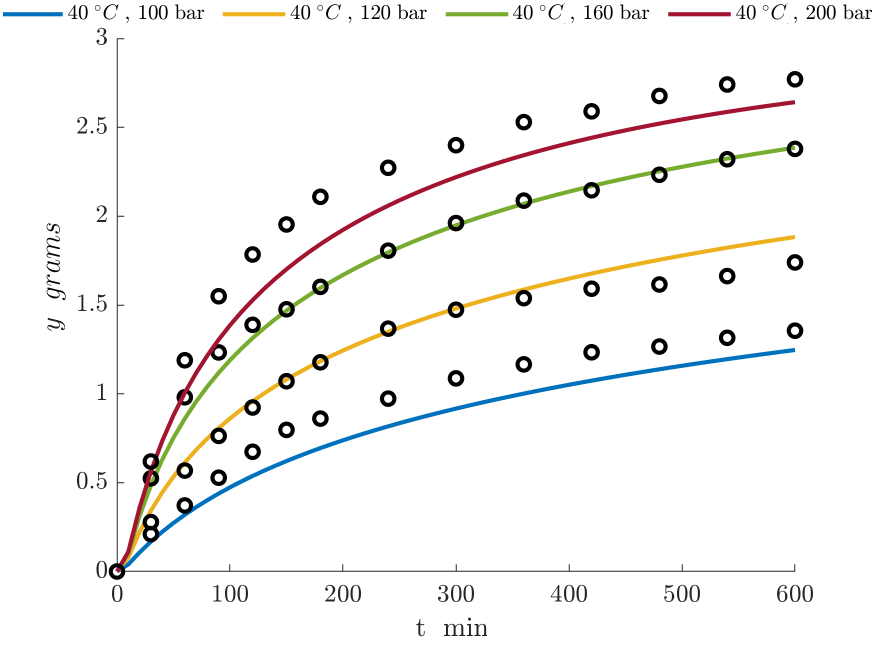
\includegraphics[trim = 0.0cm 0.0cm 0.0cm 0.0cm,clip, width=\columnwidth]{/Results_estimation/Fit_Di_Gamma_1_4_correlation_1.png}
			\caption{Simulation results obtained at $6.67\cdot 10^{-5}$ kg/s and temperature of 40 $^\circ C$}
			\label{fig: Fit_1_4_Di_Gamma_correlation}
		\end{subfigure}
		\hfill
		\begin{subfigure}{0.9\columnwidth}
			\centering
			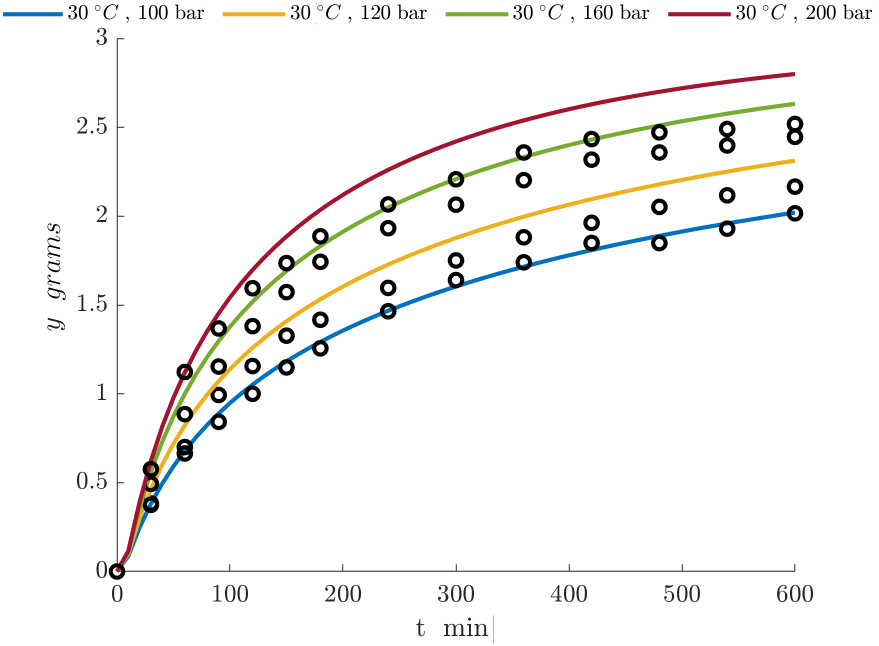
\includegraphics[trim = 0.0cm 0.0cm 0.0cm 0.0cm,clip, width=\columnwidth]{/Results_estimation/Fit_Di_Gamma_5_8_correlation_1.png}
			\caption{Simulation results obtained at $6.67\cdot 10^{-5}$ kg/s and temperature of 30 $^\circ C$}
			\label{fig: Fit_5_8_Di_Gamma_correlation}
		\end{subfigure}
		\hfill
		\begin{subfigure}{0.9\columnwidth}
			\centering
			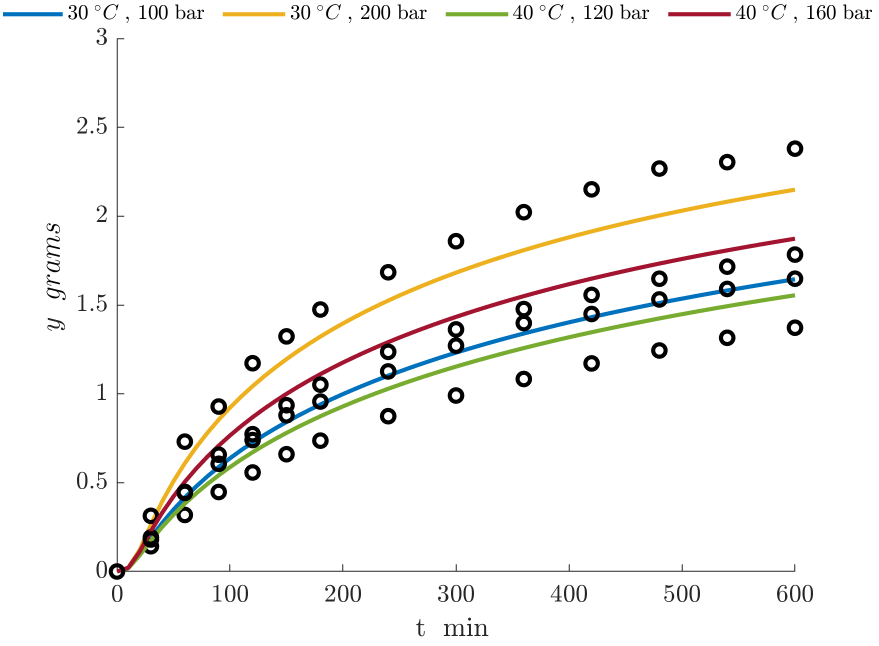
\includegraphics[trim = 0.0cm 0.0cm 0.0cm 0.0cm,clip, width=\columnwidth]{/Results_estimation/Fit_Di_Gamma_9_12_correlation_1.png}
			\caption{Simulation results obtained at $3.33 \cdot 10^{-5}$ kg/s}
			\label{fig: Fit_9_12_Di_Gamma_correlation}
		\end{subfigure}
		\caption{Simulation results from the modified model and correlations}
		\label{fig: Fit_Di_Gamma_correlation}
	\end{figure}
	
	The parameter estimation results are compared against those presented by \citet{Povh2001}, who applied the Sovova model to the same dataset. It is important to note that \citet{Povh2001} use as the initial solute mass ratio a value of 10\% above the total amount of extract for every experiment, while in this work, the initial conditions are the same for all the experiments. In contrast to this work, \citet{Povh2001} did not utilise numerical solvers but used a mix of analytical methodologies and trial-and-error procedures. \citet{Povh2001} remarked that 'the direct fitting of experimental data to Sovova's model produced parameters that could not be accepted after a careful physical interpretation of the system'. The parameters identified in this study have a physical interpretation and are within the expected range.
	
	\citet{Rahimi2011} analysed the same dataset using the desorption–dissolution–diffusion model. To decrease the number of unknown parameters, \citet{Rahimi2011} applied a set of empirical correlations. The remaining parameters were determined using a genetic algorithm to solve the parameter estimation problem for each experiment individually. Results obtained by \citet{Rahimi2011} show that the desorption–dissolution–diffusion model fails to reproduce the yield data. The main difference between the model employed by \citet{Rahimi2011} and the one in this study is the $\gamma$-function. The $\gamma$-function increases the model's flexibility by adjusting $D_i$ and allows it to obtain a better fit.
	
	\citet{Povh2001} and \citet{Rahimi2011} delivered a set of independent parameters for every experiment. This work combines the parameters obtained from each experiment to get a single correlation valid for the whole range of investigated operating conditions.
	
\end{document}













































